%%%%%%%%%%%%%%%%%%%%%%%%%%%%%%%%%%%%%%%%%
% Beamer Presentation
% LaTeX Template
% Version 1.0 (10/11/12)
%
% This template has been downloaded from:
% http://www.LaTeXTemplates.com
%
% License:
% CC BY-NC-SA 3.0 (http://creativecommons.org/licenses/by-nc-sa/3.0/)
%
%%%%%%%%%%%%%%%%%%%%%%%%%%%%%%%%%%%%%%%%%

%----------------------------------------------------------------------------------------
%	PACKAGES AND THEMES
%----------------------------------------------------------------------------------------

\documentclass{beamer}

\mode<presentation> {

% The Beamer class comes with a number of default slide themes
% which change the colors and layouts of slides. Below this is a list
% of all the themes, uncomment each in turn to see what they look like.

%\usetheme{default}
%\usetheme{AnnArbor}
%\usetheme{Antibes}
%\usetheme{Bergen}
%\usetheme{Berkeley}
%\usetheme{Berlin}
%\usetheme{Boadilla}
%\usetheme{CambridgeUS}
%\usetheme{Copenhagen}
%\usetheme{Darmstadt}
%\usetheme{Dresden}
%\usetheme{Frankfurt}
%\usetheme{Goettingen}
%\usetheme{Hannover}
%\usetheme{Ilmenau}
%\usetheme{JuanLesPins}
%\usetheme{Luebeck}
\usetheme{Madrid}
%\usetheme{Malmoe}
%\usetheme{Marburg}
%\usetheme{Montpellier}
%\usetheme{PaloAlto}
%\usetheme{Pittsburgh}
%\usetheme{Rochester}
%\usetheme{Singapore}
%\usetheme{Szeged}
%\usetheme{Warsaw}

% As well as themes, the Beamer class has a number of color themes
% for any slide theme. Uncomment each of these in turn to see how it
% changes the colors of your current slide theme.

%\usecolortheme{albatross}
%\usecolortheme{beaver}
%\usecolortheme{beetle}
%\usecolortheme{crane}
%\usecolortheme{dolphin}
%\usecolortheme{dove}
%\usecolortheme{fly}
%\usecolortheme{lily}
%\usecolortheme{orchid}
%\usecolortheme{rose}
%\usecolortheme{seagull}
%\usecolortheme{seahorse}
%\usecolortheme{whale}
%\usecolortheme{wolverine}

%\setbeamertemplate{footline} % To remove the footer line in all slides uncomment this line
%\setbeamertemplate{footline}[page number] % To replace the footer line in all slides with a simple slide count uncomment this line

%\setbeamertemplate{navigation symbols}{} % To remove the navigation symbols from the bottom of all slides uncomment this line
}

\usepackage{graphicx} % Allows including images
\usepackage{booktabs} % Allows the use of \toprule, \midrule and \bottomrule in tables

\usepackage{amsthm,amssymb}

\newcommand{\qedwhite}{\hfill \ensuremath{\Box}}

%----------------------------------------------------------------------------------------
%	TITLE PAGE
%----------------------------------------------------------------------------------------

\title[Wavelets Applications]{Wavelets and Applications} % The short title appears at the bottom of every slide, the full title is only on the title page

\author{Pankaj Patil} % Your name
\institute[UOFT] % Your institution as it will appear on the bottom of every slide, may be shorthand to save space
{
University of Toronto \\ % Your institution for the title page
\medskip
\textit{pankaj.patil@mail.utoronto.ca} % Your email address
}
\date{\today} % Date, can be changed to a custom date

\begin{document}

\begin{frame}
\titlepage % Print the title page as the first slide
\end{frame}

\begin{frame}
\frametitle{Overview} % Table of contents slide, comment this block out to remove it
\tableofcontents % Throughout your presentation, if you choose to use \section{} and \subsection{} commands, these will automatically be printed on this slide as an overview of your presentation
\end{frame}

%----------------------------------------------------------------------------------------
%	PRESENTATION SLIDES
%----------------------------------------------------------------------------------------

%------------------------------------------------
\section{Fourier Series Pitfalls} % Sections can be created in order to organize your presentation into discrete blocks, all sections and subsections are automatically printed in the table of contents as an overview of the talk
%------------------------------------------------

\begin{frame}
\frametitle{Fourier Series Pitfalls}

\begin{itemize}
    \item Fourier coefficients, and hence the Fourier series approximation, depend on all values of the function
    \item For example, if you change a function $f$ a small amount on the interval $[0, 0.01]$, it is possible that every Fourier coefficient changes. This will then have an effect on the partial sums $S_n f (\theta )$ for all values of $\theta$
    \item For a badly behaved function, such as a nondifferentiable or discontinuous one, the coefficients decrease slowly.
    \item show that the Fourier coefficients of a function go rapidly to 0 only when the functions has several continuous derivatives. Thus, we may need many terms to get a close approxima- tion, even at a point relatively far away from the discontinuity.
\end{itemize}

\end{frame}


\begin{frame}
    \frametitle{Fourier Series Pitfalls (Continued..)}
    
    \begin{itemize}
        \item The partial sums $S_n f (\theta )$ do not always converge to $f (\theta )$ when f is merely continuous.
        \item According to Gibbs’s phenomenon, $S_n f (\theta )$ will always exhibit bad behaviour near discontinuities, no matter how large n is.
        \item While we can get better approximations by using on $f (\theta )$ instead of $S_n f (\theta )$ , this will not resolve such problems as
        slowly decreasing Fourier coefficients.
    \end{itemize}
    $\implies$

    \begin{center}
        We need series expansions with better local properties.     
    \end{center}
    
    $\implies$

    \begin{center}
        Solution is Wavelets.
    \end{center}
    

    \end{frame}

    
%------------------------------------------------

%------------------------------------------------
\section{Wavelets} % Sections can be created in order to organize your presentation into discrete blocks, all sections and subsections are automatically printed in the table of contents as an overview of the talk
%------------------------------------------------

\begin{frame}
\frametitle{Wavelets}
\begin{definition}[15.1.1]
    A wavelet is a function $$\psi \in L^2 \left({\mathbb{R}}\right)$$ such that the set
    $$\{\psi_{kj}(x) = 2^{k/2}\psi(2^kx-j): k,j \in \mathbb{Z} \}$$
    forms an orthonormal basis for $L^2\left({\mathbb{R}}\right)$
\end{definition}

\begin{itemize}
\item $\psi$ is called the mother wavelet.
\item called dyadic wavelet to stress that dilations are taken to be powers of 2
\item the wavelet basis has two parameters, whereas the Fourier basis for $L^2\left({\mathbb{R}}\right)$  has only one, given by dilation alone
\end{itemize}

\end{frame}

%------------------------------------------------

%------------------------------------------------
\section{Haar Wavelets} % Sections can be created in order to organize your presentation into discrete blocks, all sections and subsections are automatically printed in the table of contents as an overview of the talk
%------------------------------------------------

\begin{frame}
\frametitle{Haar System for  $L^2\left({\mathbb{R}}\right)$ }
Start with description for $L^2([0,1])$, which will lead us to $L^2\left({\mathbb{R}}\right)$
\linebreak\linebreak
For $a < b$, let $\chi_{[a,b)}$ denote the characteristic function of $[a, b)]$.

\begin{center}
        $\phi=\chi_{[0,1)}$ and $\psi = \chi_{[0, 0.5]} - \chi_{[0.5, 1]}$
    \end{center} 
Then define,
\begin{center}
    $\{\psi_{kj}(x) = 2^{k/2}\psi(2^kx-j)$ \space\space\space for all \space\space\space $k,j \in \mathbb{Z}$
\end{center} 

We use only those functions that are supported on $[0, 1)$, namely $0 \le j < 2k$ for each
$k \ge 0$
\linebreak\linebreak
The Haar system is the family

\begin{block}{}
    \begin{center}
        $\{\phi, \psi_{kj}:k,j\ge 0 \text{ and } 0 \le j < 2^k\}$
    \end{center}
\end{block}

\end{frame}

\begin{frame}
\frametitle{ Haar System for  $L^2\left({\mathbb{R}}\right)$ (Continued..)}
Some elements of Haar System
\begin{figure}
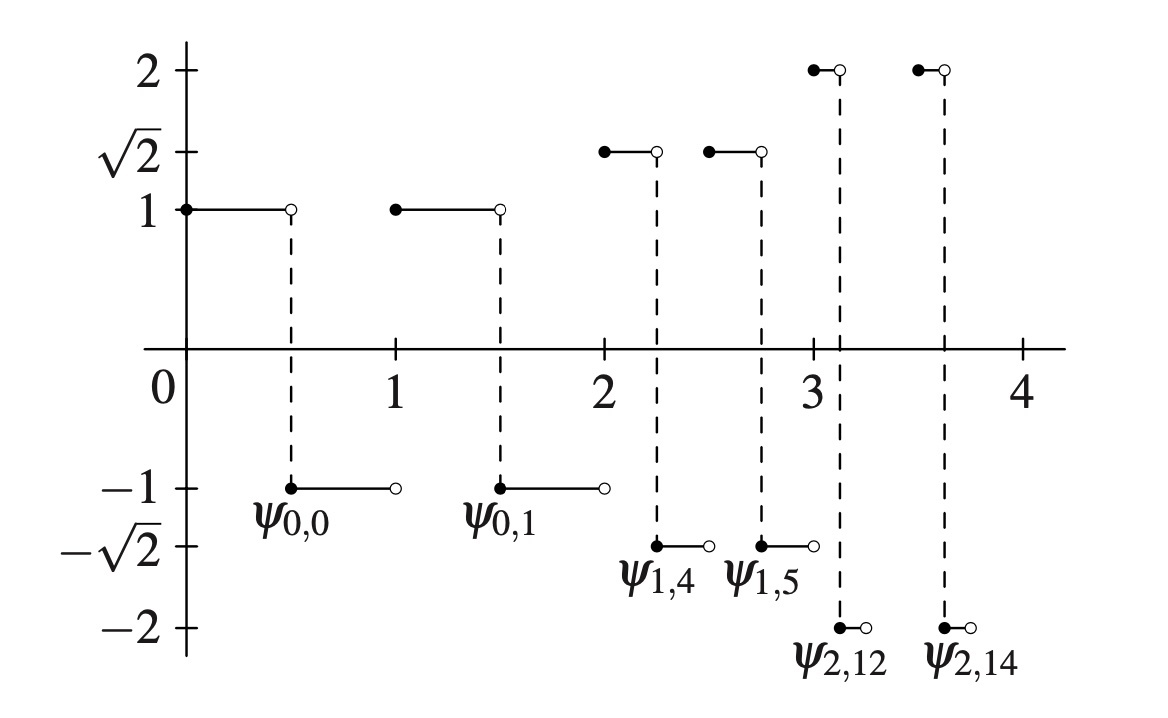
\includegraphics[width=0.8\linewidth]{haarsystem.jpg}
\end{figure}
\end{frame}


\begin{frame}
\frametitle{Haar System for  $L^2\left({\mathbb{R}}\right)$ (Continued..)}

\begin{lemma}[15.2.1]
    The Haar system is orthonormal.
\end{lemma}

\boldmath{Proof.}

Each of these functions has norm 1. 

$$\int_0^1\psi_{kj}^2(x)dx = \int_0^1 (2^{k/2})^2\psi^2(2^kx-j)dx = \int_{-j}^{2^k-j} \psi_{kj}^2(t)dt = 1$$


Now $\psi_{kj}$ and $\psi_{kj'}$ for $j \ne j'$ have disjoint supports and thus are orthogonal. 
$$\int_0^1\psi_{kj}(x)dx = 0 \text{for all } k, j$$
$\implies$ these functions are pairwise orthogonal.
\qedwhite
\end{frame}

\begin{frame}
\frametitle{Haar System for  $L^2\left({\mathbb{R}}\right)$ (Continued..)}
\textbf{Haar Coefficients}
\linebreak

Consider inner product expansion with respect to orthonormal basis and define
    $$H_nf = \langle f, \phi\rangle \phi(x) + \sum_{k=0}^{n-1}  \sum_{j=0}^{2^k-1} \langle f, \psi_{kj}\rangle \psi_{kj}(x)$$

The Haar Coefficients are the inner products $\langle f, \psi_{kj}\rangle$ used in this expansion.
\end{frame}

\begin{frame}
    \frametitle{Haar System for  $L^2\left({\mathbb{R}}\right)$ (Continued..)}

\begin{theorem}[15.2.3]
    Let $f \in L^2(0,1)$. Then $H_nf$ converges to $f$ in the $L^2$ norm.
    Consequently, the Haar system is an orthonormal basis for $L^2(0,1)$. 
    Moreover, if $f$ is continuous on $[0, 1]$, then $H_nf$ converges uniformly to $f$.
\end{theorem}

\boldmath{Proof.}

\begin{itemize}
    \item Last Part: $f$ is continuous on compact set $[0,1] \implies$ it is uniformly continuous on [0,1].
    The modulus of continuity is  given  by $$w(f;\delta)  = sup{|f(x-f(y| : |x - y| \le \delta}$$. 
    Uniform coninuity applies that $$\lim_{n \to \infty} \omega(f;2^{-n})=0$$
    Now let $x \in [j2^-n, (j+1)2^{-n})$
\end{itemize}

\end{frame}

\begin{frame}
\frametitle{Haar Wavelets}
    \begin{eqnarray*}
        \begin{split}
            |H_nf(x) - f(x)| &= |2^n\int_{j2^-n}^{(j+1)2^-n}f(t)dt-2^n\int_{j2^-n}^{(j+1)2^-n}f(x)dt| \\
            &\le 2^n int_{j2^-n}^{(j+1)2^-n}|f(t) - f(x)|dt \\
            &\le 2^n int_{j2^-n}^{(j+1)2^-n}\omega(f;2^{-n})dt \\
            &= \omega(f;2^{-n})
        \end{split}
    \end{eqnarray*}

    Hence $\Vert H_nf - f \Vert_{\infty} \le \omega(f;2^{-n})$ tends to 0. Therefore, $H_nf$ converges uniformly to $f$ on $[0, 1]$.
\end{frame}


\begin{frame}
    \frametitle{Haar System for  $L^2\left({\mathbb{R}}\right)$ (Continued..)}
    Now
    \begin{eqnarray*}
        \begin{split}
            \Vert H_nf - f \Vert_{2} &\le \left(\int_0^1 \Vert H_nf - f \Vert_{\infty}dt \right)^{1/2}\\
            &= \Vert H_nf - f \Vert_{\infty}
        \end{split}
    \end{eqnarray*}
So we have convergence in $L^2(0,1)$ norm as well.
\begin{itemize}
    \item Let  $f \in L^2(0,1)$, and $fix \epsilon > 0$. Since $f$ is the $L^2$ lmit of a sequeence of 
    continuous functions, we can find a continuous function $g$ such that $\Vert f - g \Vert_2 < \epsilon$. Choose $n$ large enough so that
    $\Vert H_ng - g \Vert_2 < \epsilon$, then
    \begin{eqnarray*}
        \begin{split}
            \Vert H_nf - f \Vert_{2} &\le \Vert H_nf - H_ng \Vert + \Vert_2 H_ng- g \Vert_2  + \Vert g -f \Vert_2 \\
            &\le \Vert H_n(f- g)\Vert_2 + \epsilon + \epsilon \\
            &\le \Vert f- g\Vert_2 +  2\epsilon \\
            &< 3\epsilon
        \end{split}
    \end{eqnarray*}
    So $H_nf$ converges to $f$  in $L^2$.
\end{itemize}
\end{frame}
    

\begin{frame}
    \frametitle{Haar System for  $L^2\left({\mathbb{R}}\right)$ (Continued..)}
    Since the orthogonal expansion of $f$ in the Haar system sums to $f $in the $L^2$ norm,
we deduce that this orthonormal set spans all of $L^2(0,1)$ and thus is a basis.

\qedwhite

\end{frame}

\begin{frame}
\frametitle{Haar Wavelets}

\begin{definition}[15.2.4]
    The Haar wavelet is the function $$\psi = \chi_{[0, 0.5]} - \chi_{[0.5, 1]}$$
    The Haar wavelet basis is the family $$\{\psi_{kj}: k,j \in \mathbb{Z} \}$$
\end{definition}

\end{frame}

\begin{frame}
\frametitle{Haar Wavelets (Continued..)}

\begin{theorem}[15.2.5]
    The Haar wavelet basis spans all of $L^2(\mathbb{R})$.
\end{theorem}

\boldmath{Proof.}\linebreak
\begin{itemize}
    \item Enough to show that any continuous function of bounded support is spanned by the Haar wavelet basis. 
    \item Each such function is the finite sum of (piece- wise) continuous functions supported on an interval $[m,m+1)$.
    \item But our basis is invariant under integer translations $\implies$it is enough to show that a function on $[0, 1)$ is spanned by the Haar wavelet basis.
    \item But Theorem 15.2.3 shows that the functions $\psi_{kj}$ supported on $[0,1)$ together with $\phi$ span $L^2(0,1)$ $\implies$ it is enough to approximate $\phi$ alone.
\end{itemize}    

\end{frame}

\begin{frame}
    \frametitle{Haar Wavelets (Continued..)}

    Consider the functions $\phi_{-k,0} = 2^{-k/2}\chi_{[0,2^{k-1})}-\chi_{[2^{k-1}, 2^k)}$ for $k \ge 1$. An easy com- putation shows that
    $$h_N := \sum_{k=1}^{N}2^{-k/2}\phi_{-k,0} = (1-2^{-N})\chi_{[0, 1]} - 2^{-N}\chi_{[1,2^N)}$$

        Thus $\Vert \phi - h_N \Vert_2 = \Vert 2^{-N}\chi_{[0,2^N)}\Vert_2 = 2^{-N/2}$. Hence $\phi$ is in the span of rhe wavelet
        basis. Therefore, the Haar wavelet basis spans all of $L^2(\mathbb{R})$.
        \qedwhite

    \end{frame}


%------------------------------------------------

%------------------------------------------------
\section{Multiresolution Analysis} % Sections can be created in order to organize your presentation into discrete blocks, all sections and subsections are automatically printed in the table of contents as an overview of the talk
%------------------------------------------------
\begin{frame}
\frametitle{Multiresolution Analysis}

\begin{block}{Objective}
    Develop a general framework to contruct other  wavelet system.
\end{block}

Define:

\begin{block}{}
    $$\phi = \chi_{[0,1)}$$
    $$\phi_{kj}(x) = 2^{k/2}\phi(2^kx - j) \text{ for all } k, j \in \mathbb{Z}$$
\end{block}

\begin{itemize}
    \item The system as is, is not orthonormal.
    \item But for each $k$, the family $\{ \phi_{kj} : j \in \mathbb{Z} \}$ is orthonormal.
\end{itemize}

Define:

\begin{block}{}
    $$V_k = span\{ \phi_{kj} : j \in \mathbb{Z} \}$$
    $$\implies V_k \subset V_{k+1}$$
\end{block}

\end{frame}

\begin{frame}
    \frametitle{Multiresolution Analysis (Continued..)}
    Some important properties of this decomosition are, 
    \begin{lemma}[15.3.1]
        Let $\phi = \chi_{[0, 1)}$, and with $V_k$ defined as before, we have
        \begin{itemize}
            \item \textbf{orthogonality}: $\{\phi(x-j) : j \in \mathbb{Z}\}$ is orthonormal basis for $V_0$.
            \item \textbf{nesting}: $V_k \subset V_{k+1}$ for all $k \in \mathbb{Z}$.
            \item \textbf{scaling}: $f(x) \in V_k$ if and only if $f(2x) \in V_{k+1}$.
            \item \textbf{desity}: $\overline{\bigcup_{k\in\mathbb{Z}}V_k} = L^2(\mathbb{R})$.
            \item \textbf{separation}: $\cap_{k\in\mathbb{Z}} V_k = {0}$.
        \end{itemize}
    \end{lemma}

\end{frame}
\begin{frame}
    \frametitle{Multiresolution Analysis (Continued..)}
    \begin{definition}[Multiresolution]
        A multiresolution of $L^2(\mathbb{R})$ with scaling function $\phi$is the sequence of subspaces
        $$V_k = span\{ \phi_{kj} : j \in \mathbb{Z} \}$$
        provided that the sequence satisfies the five properties described in the preceding lemma.
    \end{definition}

    The function $\phi$ is sometimes called a father wavelet.

    \begin{block}{}
        Orthogonality
        $$\langle \phi_{kj}, \phi_{kl}\rangle = \int_{-\infty}^{\infty} 2^k\phi(2^kx-j)\phi(2^kx-l)dx = \int_{-\infty}^{\infty} \phi(t-j)\phi(t-l)dt = \delta_{jl}$$
    \end{block}

\end{frame}

\begin{frame}
    \frametitle{Multiresolution Analysis (Continued..)}
    \begin{theorem}[15.4.2]
        Let $\phi$ be the scaling function generating a multiresolution $\{V_k\}$ of $L^2(\mathbb{R})$ 
        with scaling relation $\phi(x) = \sum_{j=-\infty}^{\infty}a_j\phi(2x-j)$. Define
$$\psi(x) = \sum_{j=-\infty}^{\infty} (-1)^ja_{j-1}\phi(2x-j)$$
Then $\psi$ is a wavelet that generates the wavelet basis $\{\psi_{kj} : k, j \in \mathbb{Z}\}$ such that
$W_k = span\{ \psi_{kj} : j \in \mathbb{Z} \}$ for each $k \in \mathbb{Z}$

    \end{theorem}

\end{frame}

%------------------------------------------------
\section{Daubechies Wavelets} % Sections can be created in order to organize your presentation into discrete blocks, all sections and subsections are automatically printed in the table of contents as an overview of the talk
%------------------------------------------------
\begin{frame}
\frametitle{Daubechies Wavelets}

\begin{itemize}
    \item Haar wavelets do a good job of approximating functions that are locally constant
    \item Can approximate continuous functions if we use a wavelet that also satisfies $$\int x\psi(x) dx = 0$$ It is called first moment of $\psi$.
\end{itemize}

\begin{theorem}[15.5.1]
    There is a continuous function $\phi$ of compact support in $L^2(\mathbb{R}) $
    that generates a multiresolution of $L^2(\mathbb{R}) $such that the associated wavelet $\psi$ is continuous, 
    has compact support, and satisfies $$\int \psi(x) dx = \int x\psi(x) dx = 0$$.
\end{theorem}

\end{frame}

\begin{frame}
    \frametitle{Daubechies Wavelets (Continued..)}
    
    \begin{itemize}
        \item This is called Daubechies scaling function.
        \item It has all the good properties we wanted.
        \item It has support on $[0,3]$.
        \item The graph  of $\phi_4$ and $\phi_5$
    \end{itemize}

    \begin{figure}
        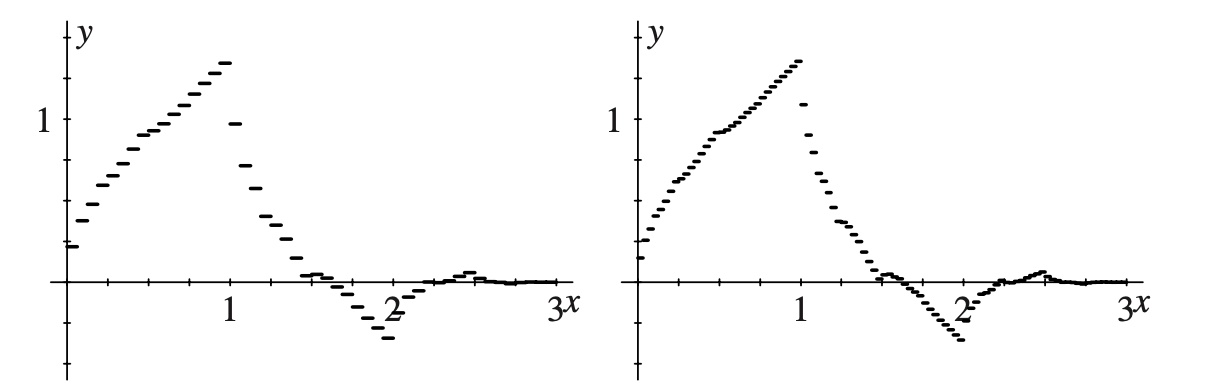
\includegraphics[width=0.8\linewidth]{daubechies.jpg}
    \end{figure}
    
\end{frame}
    
%------------------------------------------------
%------------------------------------------------
\section{Function Approximation using Haar Wavelets} % Sections can be created in order to organize your presentation into discrete blocks, all sections and subsections are automatically printed in the table of contents as an overview of the talk
%------------------------------------------------

\begin{frame}
\frametitle{Function Approximation using Haar Wavelets}
$f(x) = x^3$ approximation  using Haar Wavelets
\begin{figure}
    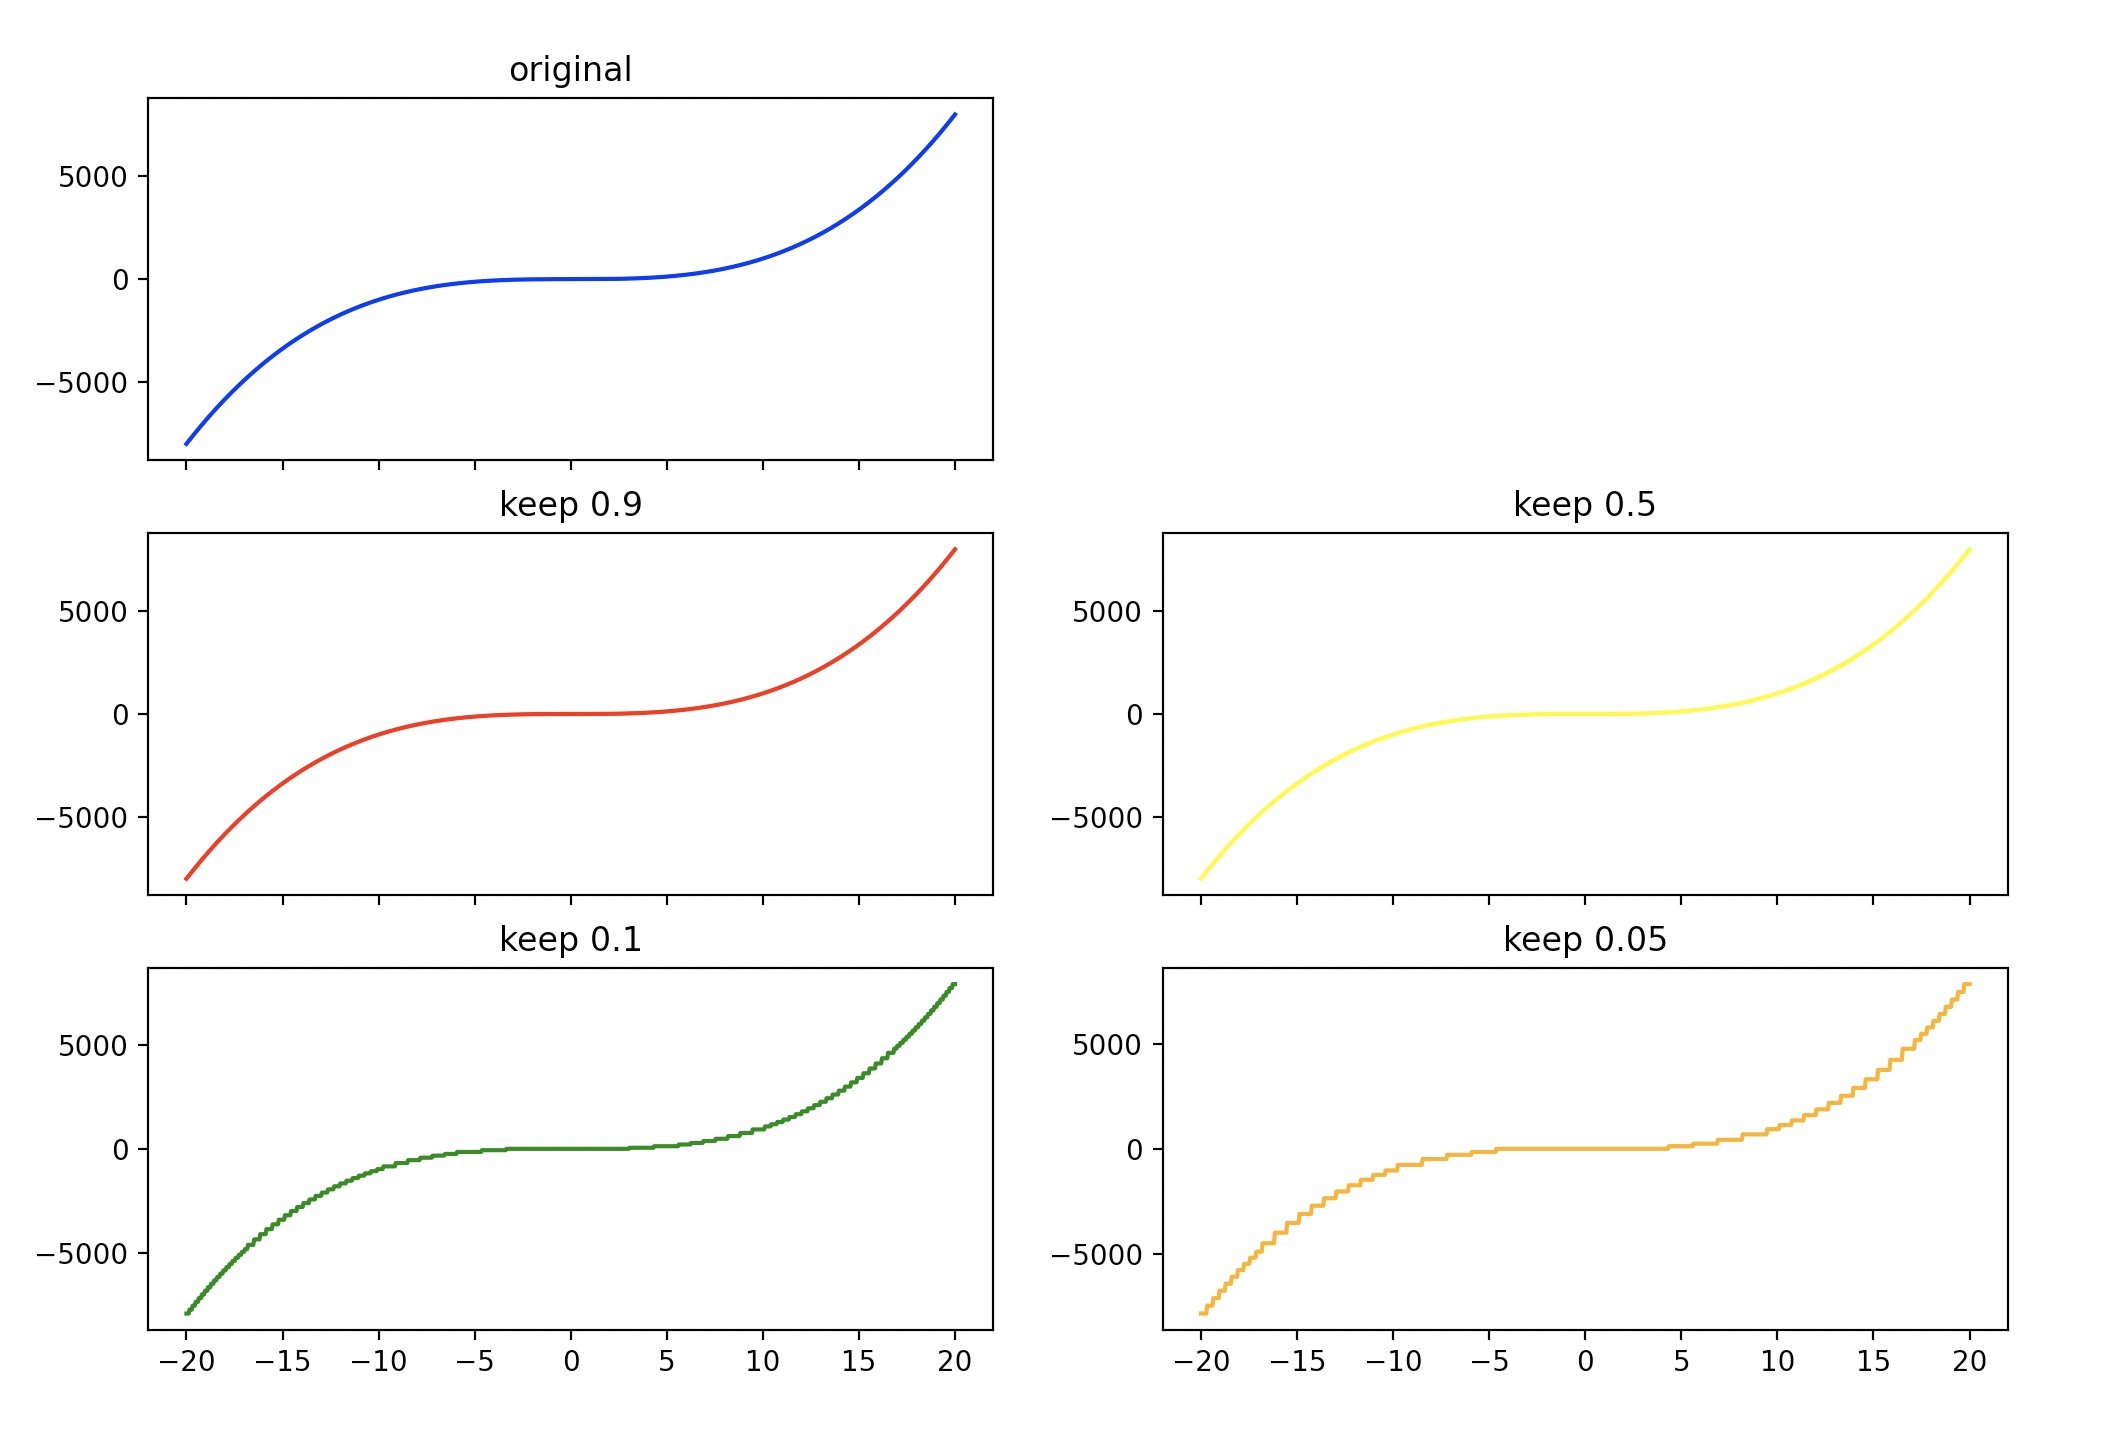
\includegraphics[width=0.8\linewidth]{x3.jpg}
\end{figure}
\end{frame}

%------------------------------------------------
%------------------------------------------------
\section{Image Compression using Daubechies Wavelets} % Sections can be created in order to organize your presentation into discrete blocks, all sections and subsections are automatically printed in the table of contents as an overview of the talk
%------------------------------------------------

\begin{frame}
\frametitle{Image Compression using Daubechies Wavelets}

\begin{itemize}
    \item Signals and Images have lot of redundant data because of correlation within th data.
    \item If signal is continuous, then we can store only the value at certain time and then only increments to it, so that the original signal can be reconstructed.
    \item This reduces storage requirements and is an example of data compression.
    \item In case of images, the same principle follows. The wavelet expansion for images can generate many coefficients that are insignificant and can be discarded without losing must in terms of quality of the reconstructed image.
    \item Caution: more coefficients discarded more is the error.
\end{itemize}
\end{frame}


\begin{frame}
    \frametitle{Image Compression using Daubechies Wavelets}
    \begin{figure}
        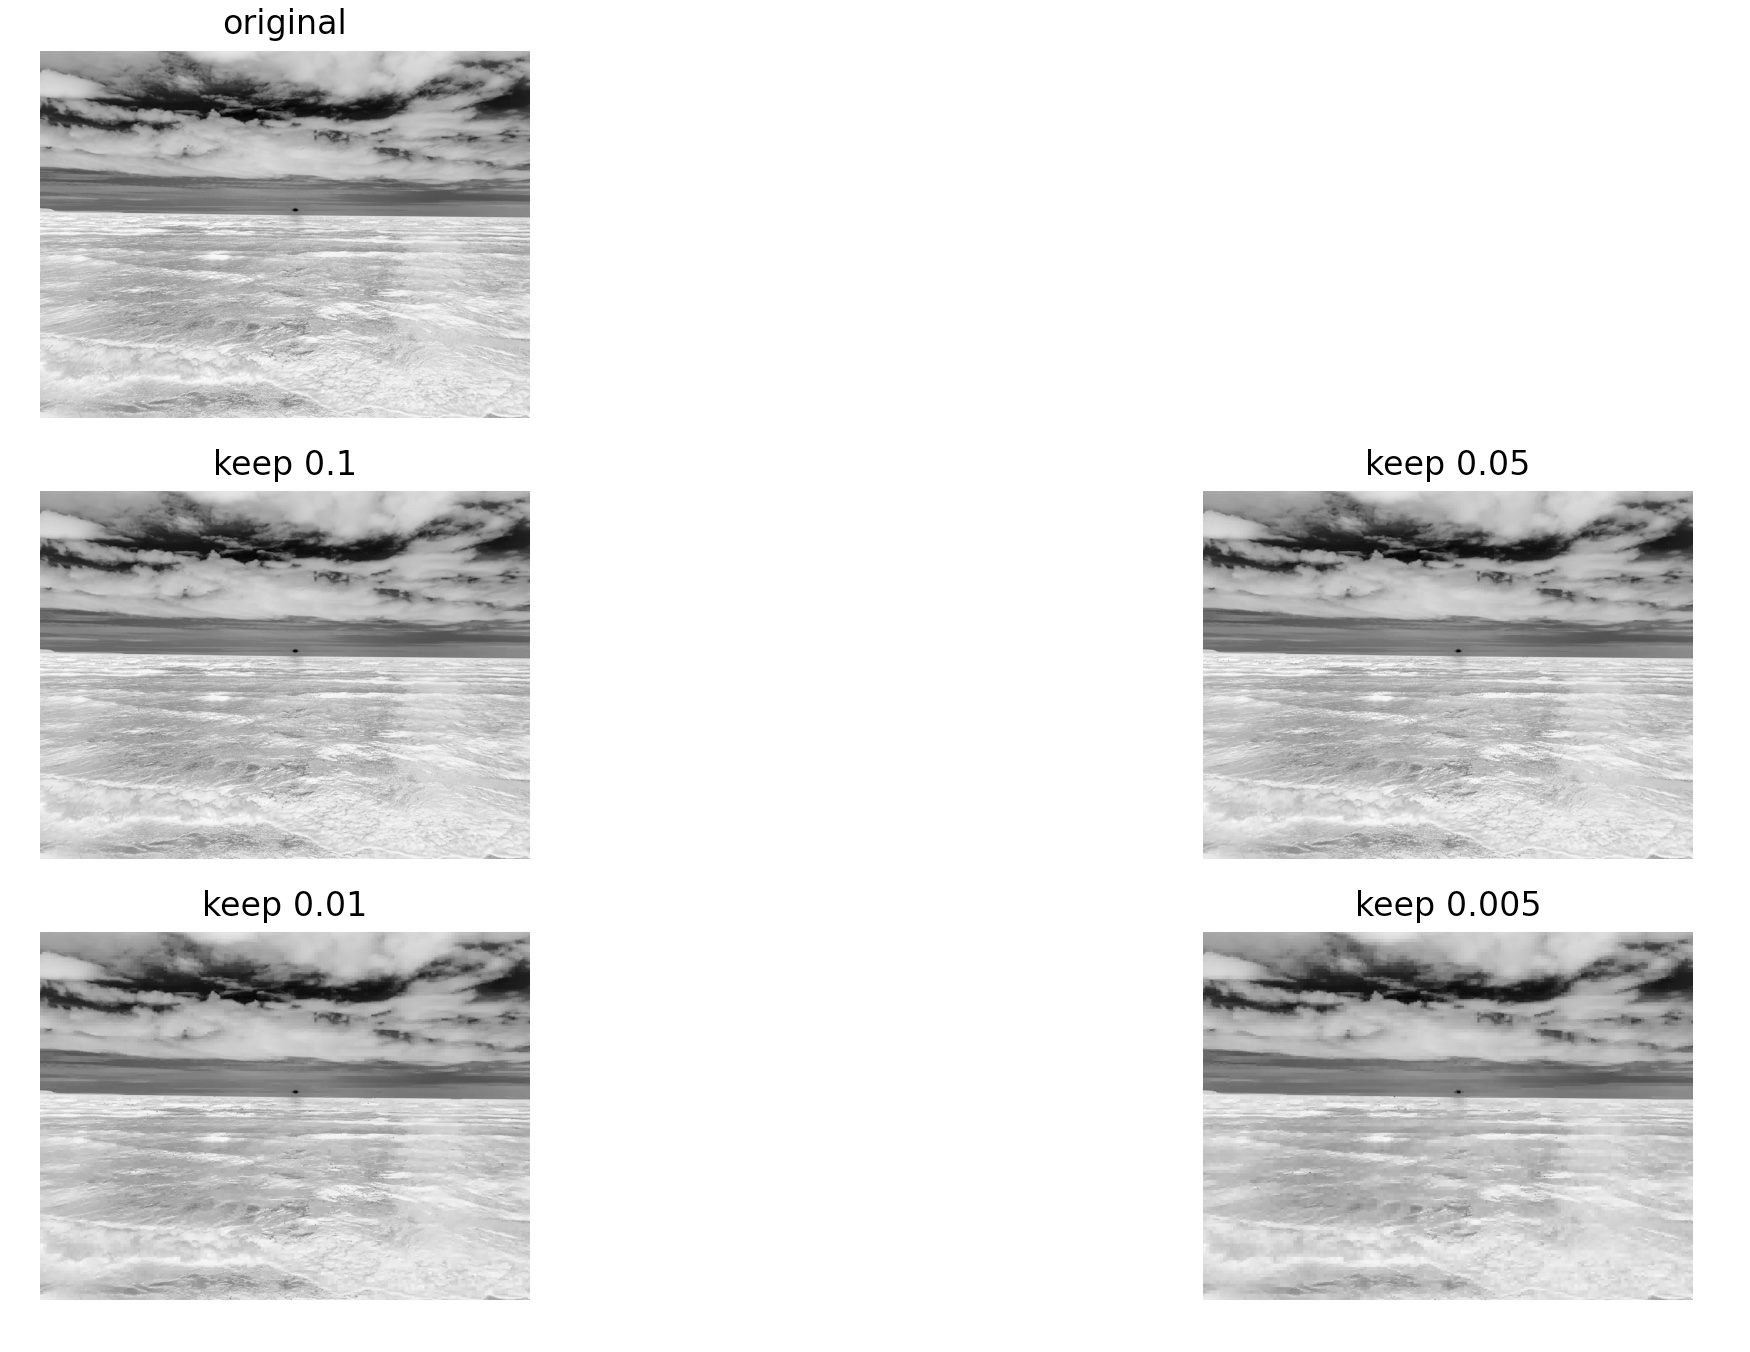
\includegraphics[width=0.8\linewidth]{image.jpg}
    \end{figure}
    \end{frame}
    

%------------------------------------------------

\begin{frame}
\Huge{\centerline{Thank You.}}
\end{frame}

%----------------------------------------------------------------------------------------

\end{document} 